\documentclass[10.5pt, a4paper, twoside]{article}
\providecommand{\abs}[1]{\lvert#1\rvert}
\setlength{\topmargin}{-1.25in}
\setlength{\footskip}{0.75in}
\setlength{\textheight}{10in}

\usepackage[margin=2.5cm]{geometry}
\usepackage{amsfonts}
\usepackage{amsmath}
\usepackage{amssymb}
\usepackage{graphicx}
\usepackage{enumerate}
\usepackage{color}
\usepackage{float}
\usepackage{setspace}
\usepackage{tabularx}
\setlength{\extrarowheight}{5pt}
\usepackage[labelfont=bf]{caption}
\usepackage{subfig}

%%%% BIBLIO

\usepackage[backend=bibtex]{biblatex}

%%%% GLOSSARY STUFF

\usepackage[intoc]{nomencl}

\renewcommand{\nomname}{Glossary}
\renewcommand{\nomlabel}[1]{\textbf{#1}}
\makenomenclature

%\singlespacing
\onehalfspacing
%\doublespacing
%\setstretch{1.1}

\setlength\parindent{0pt}

\newenvironment{packed_itemize}{
\begin{itemize}
  \setlength{\itemsep}{1pt}
  \setlength{\parskip}{0pt}
  \setlength{\parsep}{0pt}
}{\end{itemize}}

\definecolor{dkgreen}{rgb}{0,0.6,0}
\definecolor{gray}{rgb}{0.5,0.5,0.5}
\definecolor{mauve}{rgb}{0.58,0,0.82}

\newcommand{\vecthree}[3]{\left(\!\!{\scriptsize\begin{array}{c}#1\\#2\\#3\end{array}}\!\!\right)}
\newcommand{\vectwo}[3]{\left(\!\!{\scriptsize\begin{array}{c}#1\\#2\end{array}}\!\!\right)}
\newcommand{\HRule}{\rule{\linewidth}{0.5mm}}

\newcommand{\ggather}[1]{\begin{gather}#1\end{gather}}
\newcommand{\nggather}[1]{\begin{gather}#1\end{gather}}

\newcolumntype{C}{>{\centering\arraybackslash}X}
\newcolumntype{L}{>{\raggedright\arraybackslash}X}

\addbibresource{sources.bib}

\begin{document}
%
%\title{ \bf \huge Development of a 12.4 GHz Bandwidth Frequency Offset Locking Unit for Two-Laser Systems}
%\author{Steve Novakov }
%\date{}
%
%\maketitle

\begin{titlepage}
\begin{center}

% Upper part of the page. The '~' is needed because \\
% only works if a paragraph has started.

% Title
\HRule \\[0.4cm]
{ \huge \bfseries Pound-Drever-Hall Servomechanism with an Atomic Referece for Frequency Stabilization of a Master Laser \\[0.4cm] }

\HRule \\[1.3cm]

{ \huge \bfseries Final Recommendation Report \\[1.3cm] }

% Author and supervisor

\begin{tabularx}{\linewidth}{lXr}
  \Large \emph{Authors:} & & \Large \emph{Sponsor:} \\
  \Large \textsc{Steve Novakov} & & \Large \textsc{Dr.~Kirk Madison} \\
  \Large \textsc{Jeff Taylor}  & & \\
\end{tabularx}

\vfill

\textsc{\LARGE ENPH 479}\\[0.3cm]
\textsc{\LARGE Engineering Physics}\\[0.3cm]
\textsc{\LARGE University of British Columbia}\\[0.3cm]

\vfill

\textsc{\Large Group 1472}\\[0.3cm]
\textsc{\Large Project 33}\\[0.3cm]

\vfill

% Bottom of the page
{\large \today}

\end{center}
\end{titlepage}
\newpage

%%%%%%%%%%%%%%%% EXECUTIVE SUMMARY

\newpage
\section*{Executive Summary}

This project, sponsored by the UBC Quantum Degenerate Gases
Laboratory - Madison Group, aims to build and characterize a high
fidelity, small linewidth, laser frequency locking system based on the
Pound-Drever-Hall (PDH) locking method. The QDG laboratory 
specializes in manipulation of atomic and molecular gases with
optical systems that implement some form of laser cooling. To 
efficiently cool or manipulate these ensembles, the lasers involved
must be tuned to specific frequencies, often corresponding to atomic
transitions, and have as small a linewidth as possible. Any increase 
in the fidelity of the probing or pumping lasers often has immediate
impact on the quantity of atoms that can be trapped/cooled, and the 
lowest attainable temperature in a trap. Specifically, in some cases, 
the linewidth must be as small as possible around the resonant frequency 
of a transition. \\

Existing systems at the sponsors' laboratory are already based 
on the PDH method, but use a slightly different approach. Both the 
existing and proposed systems will lock to a frequency-discriminating 
object, specifically a vapor cell of the relevant atomic species. The
existing locking unit makes use of an Acousto-optic Modulator (AOM), a 
device which takes a seeding beam from a diode laser as an input and, 
through acoustic vibration generated by a piezo-electric transducer, 
produces a Doppler-shifted diffraction pattern. This pattern is then 
sent through a vapor cell (though commonly, an external cavity is used), 
and the filtered beam is coupled into a photosensor and mixed/processed 
to produce an error signal. This signal is then used by the diode laser 
control system to lock to the resonance frequency of the selective 
element. Unfortunately, due to mechanical limitations of the AOM device, 
the dithering frequency of the modulated beam output, which drives the 
resolution of the error signal, is quite small, approximately 200 kHz. 
Furthermore, the processing required to use this signal decreases the 
settling time further, approximately 10-20 fold to 10 kHz [maybe cite 
something here, rather than relying on just Kirk's description]. This 
results in a large setting time for the control circuit, which 
necessarily increases the linewidth of the laser.  \\

To increase the bandwidth of the locking circuit and therefore 
reduce the linewidth of the master laser, a PDH unit based around an 
Electro-Optic Modulator (EOM) will be built, and its performance will be 
benchmarked to the existing AOM locking unit. An EOM, commonly known as 
a "Pockels Cell" as it exploits the Pockels Effect, is a physical medium 
which phase modulates a beam in its direction of propagation at a 
driving frequency. The output beam has the same fundamental as the input 
beam, as well as a well-defined spectrum of side-bands. This composite 
beam is then sent through the frequency selective unit and, again, mixed 
to produce an error signal. The primary difference, relative to the AOM 
unit, is that the mixing technique is slightly different and, more 
importantly, that the dithering frequency is significantly higher. Some 
EOM units can handle modulation at over 100 MHz, though, for this 
project, a frequency of 10-20 MHz will likely be sufficient. This 
drastic increase in the control loop bandwidth will result in a much 
smaller linewidth for the master laser, and, ultimately, higher 
experimental efficiency. \\

There will be three primary stages to this project. First, the 
existing system will be evaluated for key parameters such as laser 
linewidth, and the relationships between factors like the noise floor,
modulation frequency and the transfer function of the frequency selective
unit will be quantified and recorded as benchmarks. This information 
will be used to spec various optical and electronic components for the
locking unit. Second, the locking unit will be designed to fit on an 
optical breadboard of convenient size. It is possible that a custom CCA 
will have to be designed to control the EOM, generate the error signal, 
and interface with laboratory computers. Third, the built locking unit 
will be tested and benchmarked against the metrics obtained from the 
existing setup. The target linewidth of the master laser will be determined during the first design stage.
 


%%%%%%%%%%%%%%%% TOC / FIGURES / TABLES
\newpage
\tableofcontents
\newpage
\listoffigures
\listoftables

%%%%%%%%%%%%%%% GLOSSARY

\newpage
\section*{Glossary}

\begin{tabularx}{\linewidth}{lX}
  {\bf CCA} & Circuit Card Assembly: includes a PBC and all of its components,
  sometimes encludes complimentary mechanical components as well. \\
  {\bf DDS} & Direct digital synthesizer: a synthesizer used for creating
  arbitrary waveforms from a reference clock. \\
  {\bf EMI} & Electromagnetic Interference: two types: radiated and conducted.\\
  {\bf FO (Receiver)} & Fiber Optic (photosensor unit for detecting fiber optic
  signals).  \\
  {\bf MOT} & Magneto-optical Trap. \\
  {\bf PCB} & Printed Circuit Board. \\
  {\bf PSU} & Power supply unit. \\
  {\bf RF} & Radio Frequency. Used to refer to components or systems which
  operate in the 3 kHz - 300 GHz regime. \\
  {\bf ROSA} & Receiver optical sub-assembly \\
  {\bf SMPS} & Switch-mode Power Supply: a power supply that utilizes
  energy conversion principles such as buck, boost, buck-boost, etc, typically
  driven at a particular switching frequency, as per the demands of the
  application. \\
  {\bf VCO} & Voltage Controlled Oscillator, may be crystal or PLL based. \\
  {\bf $V_{PP}$} & Peak-to-peak voltage: the full range of voltage of a
  particular waveform.
\end{tabularx}

%%%%%%%%%%%%%%%% BACKGROUND/MOTIVATION/OBJECTIVES

\newpage
\section{Introduction}

\subsection{Laser Locking}

The ability to lock a laser to a very specific frequency is of great importance to the UBC Quantum Degenerate Gases Laboratory.  They use these optical systems to laser cool atomic and molecular gases.  This requires a very narrow linewidth on the laser, and a specific frequency.  Any improvement in the frequency precision of the laser will increase the quantity of atoms that can be trapped or cooled, as well as the attainable temperatures in a trap.  Often, this frequency must be very close to the natural transitions of the gas.

One way to acquire such a system is to pass the beam through a gas.  The gas has transitions at particular energies, which can be detected by sweeping the laser (or an associated probe beam).  When doing this, the gas atoms will absorb photons at the corresponding frequencies, which will appear on a spectrum analyser.  However, since the gas is at room temperature, the broad absorption dip will have a bandwidth of about 1GHz, which is too wide to lock a laser to.

\subsection{Doppler Effects}

Since the gas atoms are moving in different directions, some atoms will be moving towards the laser beam, and other atoms will be moving away from it (some will be in between, of course).  As a result, if a single laser is used, the atoms moving towards the laser will perceive a higher frequency, and thus will excite at lower frequencies than the resonance frequency.  The opposite is also true.  If the absorption-vs-frequency curve is measured for a laser passed through the gas, there is a wide smear that is approximately 1GHz wide \cite{madison14}.  This makes the apparent spectrum of the gas much wider, and thus, much harder to lock a signal to.  This is depicted in Figure~\ref{fig:doppler}.

A major improvement is to redirect the single frequency laser around the sample, to the opposite side.  Now, when the sweep laser is at the same frequency as the pumping laser, its light will not be absorbed by the atoms with zero horizontal velocity.  This creates a Doppler-cancelled feature, which is about 10--100MHz wide.

\subsection{Acousto-Optic Modulator}

One way to modulate the frequency of the beam is to use an *acousto-optic modulator* (AOM).  An AOM is a device that acoustically varies its shape, adjusting the distance the light has to travel to reach its destination.  By modulating this at a frequency $\Omega$, we produce a beam of light with sidebands at $\omega + \Omega$ and $\omega - \Omega$, where $\omega$ is the original frequency of the laser. These devices use acoustics, so they are limited by the mechanical properties of the device.  As a result, the AOM in use by the sponsor effectively has a maximum modulation frequency of about 200kHz.  The acousto-optic modulator also creates a shift in the frequency of the carrier wave.  This shift needs to be cancelled out in a later stage of the system.

\subsection{Electro-Optic Modulator}

An \emph{electro-optic modulator} (EOM), is a device that uses an electric field to modulate the phase of a light wave.  These devices exploit the \emph{Pockels effect}, whereby the speed of light in a crystal is affected by the presence of an electric field.  Therefore, by adjusting the electric field in the crystal, the phase (and ultimately frequency spectrum) of the beam can be adjusted.  The EOM does \emph{not} shift the carrier frequency, unlike an AOM.

Unfortunately, the Pockels effect requires fairly large driving voltages, on the order of hundreds of volts.  Some manufacturers provide a full EOM solution, with built-in amplifier, to make their equipment easier to use, making an external high-voltage amplifier unnecessary.

\subsection{The Pound-Drever-Hall Method}

Optical frequencies generally exceed 100THz. It is generally not possible to
extract information at these frequencies using conventional
electronic measurement equipment.  Systems make use of
schemes that down-mix these optical signals into RF range, which are then
processed via conventional means (RF electronics and digital systems). \\

The Pound-Drever-Hall method makes use of phase-modulated light to measure an
optical response and down-mix it into RF range.  This signal is then mixed again with the same oscillator to produce a DC signal.  This signal is a function of the derivative of the absorbance spectrum of the vapour cell.  Changing the modulation frequency varies the resolution of this derivative function.  At extremes, this derivative function is either small and featureless, or is excessively noisy and not useful. \\

This method is used to lock to extrema of absorption spectra.  In an atomic gas, these features are typically transition and crossover resonances \cite{maguire2006}. Carefully selecting a modulation frequency to obtain a useful error signal about a point of interest is a principal challenge of implementing this method.

\begin{figure}
    \centering
    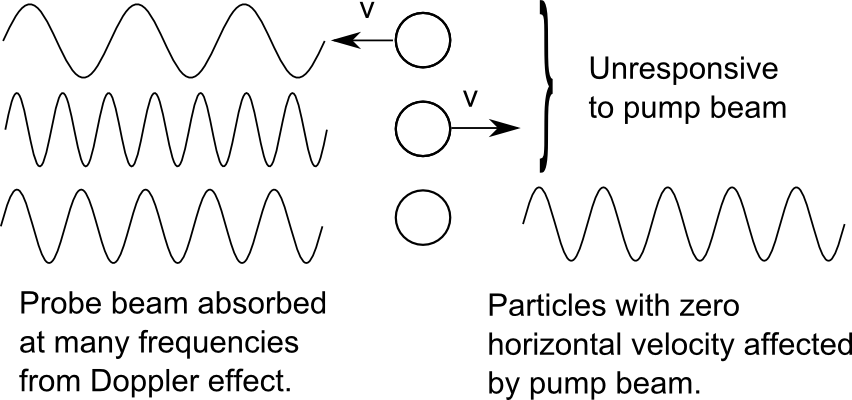
\includegraphics[width=9cm]{doppler.pdf}
    \caption{Doppler effect demonstration.  Probe beam is absorbed across a wide frequency range, but only the non-Doppler-shifted particles are affected by both beams from left and right.}
    \label{fig:doppler}
\end{figure}



%%%%%%%%%%%%%%%% BACKGROUND THEORY

\newpage
\section{Theory and Implementation} \label{sec:theory}

To gain an understanding of the motivations behind this project it is worthwhile to discuss both prior work done with the PDH method, and the motivations behind using it to lock to an atomic source.  The PDH method is often used to lock a laser to an actuated cavity \cite{black1998}.  The Madison group primarily performs laser cooling experiments on Lithium and Rubidium gas.  They need to precisely set laser frequencies at or near key atomic transitions. For example, the Rb87 $5S_{1/2} \rightarrow 5P_{3/2}$ or "D2" transition is the focus of this project.  The closer a laser's frequency is to a desired transition and the smaller the linewidth of that laser, the more efficient any excitation will be.  This has a direct impact on experimental outcome.

\subsection{Brief Overview of Saturated Absorption Spectra}

Using a vapour cell as a frequency selective feature means that the error signal
is being generated from the absorption absorption spectrum of the particular
vapour. To understand what this spectrum looks like, it is sufficient to do a
basic analysis using semi-classical derivations. Because the gas is not
collimated, and is sufficiently hot (room temperature), the constituent
atoms are moving in every direction with the typical Maxwell-Boltzmann speed
distribution. As the primary concern is exposure to a laser beam, the
velocity classes to be considered here are distributed in one direction only,
here referred to as "z":
\begin{gather}
  \rho(v_z) = \sqrt{\frac{m}{2\pi k_B T}} e^{\frac{-m v_z^2}{2k_B T}}
\end{gather}
Each velocity class absorbs the incident beam at a rate that is dependent on
how far it is from a transition resonance. Furthermore, if the atoms are not
stationary, then the incident light is Doppler shifted. This results in the
standard Lorentzian absorption profile with a Doppler correction:
\begin{gather}
  F(\nu, v_z) = \frac{\Gamma / 2 \pi}{(\nu - \nu_0 + \nu_0 v / c)^2 +
  \Gamma^2 / 4}
\end{gather}
where $\nu_0$ is the transition resonance, and $\Gamma$ is the transition
linewidth. Putting these two terms together, and integrating over all velocity
classes in the "z" direction results in a term known as \emph{optical depth}:
\begin{gather}
  \tau(\nu) = \int_{-\infty}^\infty F(\nu, v_z) \rho(v_z) dv_z
\end{gather}
which is a measure of the sample's tendency to absorb an incident photon of
frequency $\nu$. \\

An incident laser beam will enter the vapour cell and be absorbed according to
the optical depth of the medium. However, photons will be re-emitted in a random
direction and so the intensity of the incident beam will be attenuated in the
original propagation direction, depending on its frequency and the quantity
of the medium it has passed through:
\begin{gather}
  I(\nu, z) = I_0 e^{-\tau(\nu)\cdot z}
\end{gather}
Plotting $I/I_0 (\nu, L)$, for some fixed vapour cell length L, and for
values corresponding to the Rb87 D2 transition generates a
a fairly broad absorption spectrum that is essentially Gaussian with a width of approximately 1GHz \cite{maguire2006}.  Using the PDH method to lock to this feature
alone is not atttractive as it generates a very low slope about the null locking
point. If a laser is needed to specifically excite a particular hyperfine
transition, for example, this locking method will not be sufficient. \\

To generate a feature which is suitable for tight locking, a profile known as a
saturated absorption spectrum is generated by exciting the vapour cell with
a beam propagating in the opposite direction of the master laser beam. This beam
is referred to as the "pump" beam, as it serves to pump some of the atomic
population into the excited state and make it innaccesible to the original beam,
hereby referred to as the "probe". The pump beam is normally derived from the
probe beam itself. This results in an additional effect that starves the probe
beam of accessible atoms. For a simple two level system, this can be written as:
\begin{gather}
  S(I_p, \nu, v) = \tau_0 \frac{\nu_0}{c} (P_1 - P_2) =
    \tau_0 \frac{\nu_0}{c} (1 - 2 P_2)
\end{gather}
where $P_1$ and $P_2$ are the ground and excited state population, respectively,
and the other terms are simply normalization constants. An expression for
$P_2$ can be derived that depends on the pump beam intensity, $I_p$, frequency,
$\nu$, here the same as the probe, and the linewidth of the transition
\cite{maguire2006}:
\begin{gather}
  P_2(I_p, \nu, v) = \frac{ (I_p/I_{sat})/2}{1 + (I_p/I_{sat}) +
    4(\nu - \nu_0 - \nu_0 v/c)^2/\Gamma^2}
\end{gather}
Implementing this factor into the prior calculation gives a corrected optical
depth:
\begin{gather}\label{eq:corr_opt_depth}
  \tau'(\nu) = \int_{-\infty}^\infty S(I_p, \nu) F(\nu, v_z) \rho(v_z) dv_z
\end{gather}
The resultant saturated spectrum is shown in \textbf{Figure~\ref{fig:rb87d2abs}}
, for a variety of $I_p$. The emergent feature at the transition resonance is
referred to as a "Doppler-free" feature. This nomenclature refers to the fact
that the velocity class that is most exposed to both the pump and probe beam
is the class around $v_z = 0$. This results in a decrease in probe beam
absorption from that class, and therefore, a higher transmission ratio.
This feature is shown in more detail in \textbf{Figure~\ref{fig:rb87d2abs_closer}}.

\begin{figure}
  \centering
  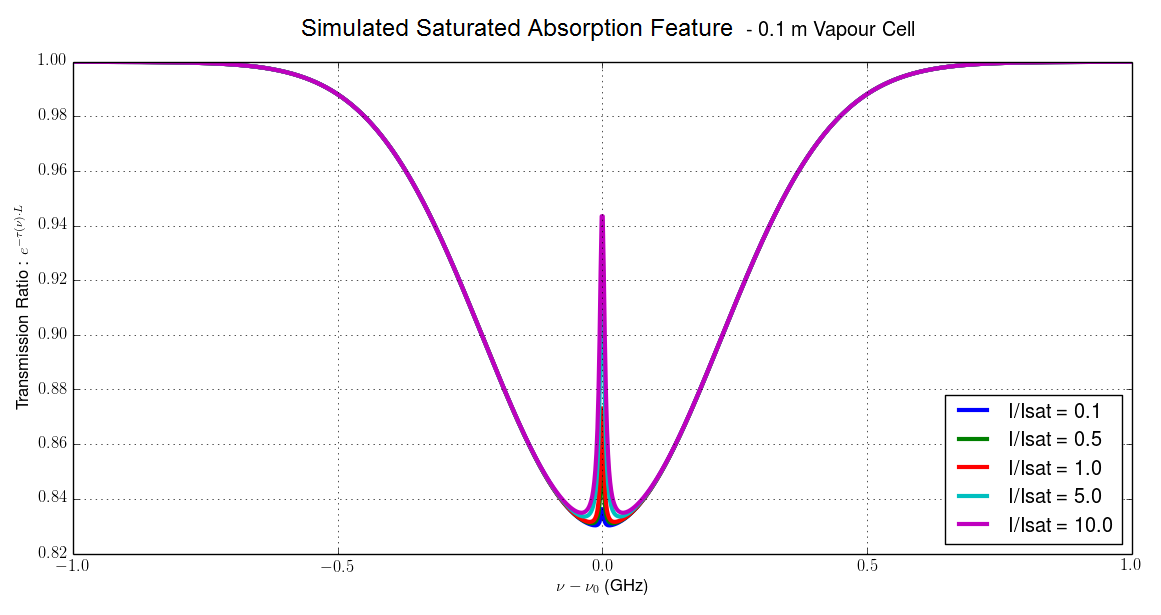
\includegraphics[scale=0.5]{rb_D2_single_absorption.png}
  \caption{Transmission ratio of probe beam through a 0.1m long cell of Rubidium
  gas, near the D2 feature. Optical depth is calculated as shown in
  \textbf{(\ref{eq:corr_opt_depth})},
  and all hyperfine splitting is ignored, (assumed 2-level system) for
  simplicity. The spectrum is plotted for a variety of pump beam intensities
  showing the saturating effect on the velocity classes near $v_z = 0$ at
  resonance.}
  \label{fig:rb87d2abs}
\end{figure}

\begin{figure}
  \centering
  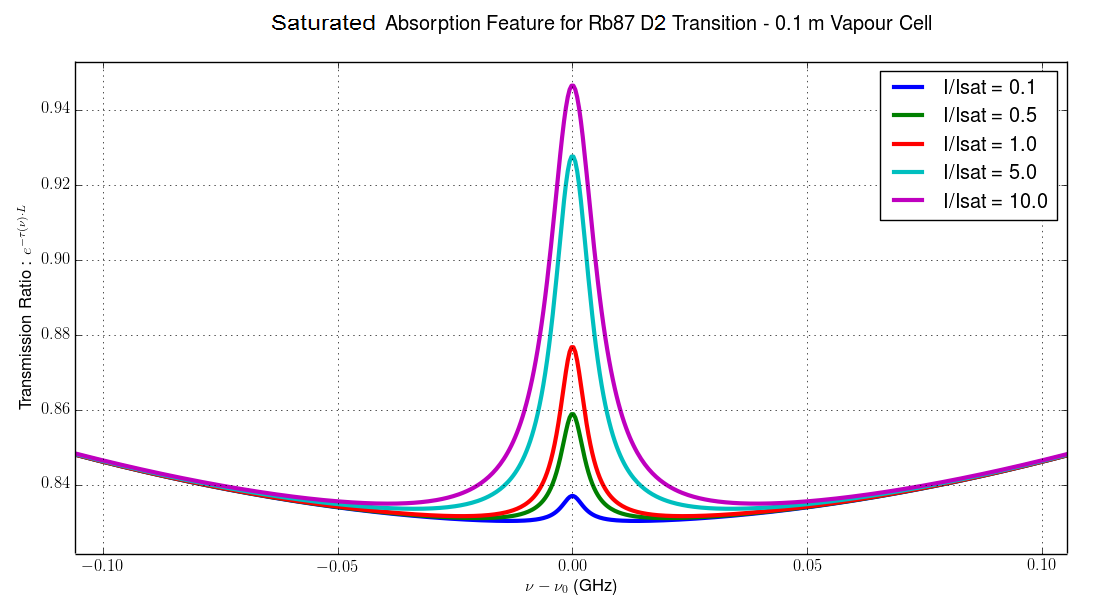
\includegraphics[scale=0.5]{rb_D2_single_absorption_resonance.png}
  \caption{Closer view of \textbf{Figure~\ref{fig:rb87d2abs}}, near the
  resonance.}
  \label{fig:rb87d2abs_closer}
\end{figure}

The model presented here is naive. The Rb87 $5P_{3/2}$ state has 4 hyperfine
levels, and transition from the ground state is goverened by the standard
selection criteria (\cite{steckrb87}, see Figure 2). This produces a much more
complicated absorption feature, with multiple transition and crossover
resonances (\cite{maguire2006}, see Figure 3). Calculating an optimal modulation
frequency for locking about one of the predominant resonance features inside the
Rb87 D2 spectrum can be done with detailed quantum mechanical analysis. It is
unclear if this is necessary, or whether the locking unit should simply be built
with an appropriate phase modulation bandwidth such that heuristic tuning can
attain an optimal result.

\subsection{Optical Phase Modulation}

As it is not possible to process optical signals in the THz range electronically,
it is common to modulate these signals to produce a spectrum about the carrier,
and then down-mix them to RF signals to extract the relevant information.
For optical signals, this is typically done with either an AOM or an EOM. From
a mathematical standpoint, the only difference between the two methods is
what phase modulation depths and frequencies are physically attainable. \\

With AOMs, which use acoustic waves to Doppler shift a beam in the transverse
direction of propagation, there is a distinct tradeoff between modulation
frequency and the resultant power of the outgoing beam.  The AOMs in current use by the Madison Group only have a useful
modulation frequency of approximately 200 kHz \cite{madison14}. \\

The modulation frequency of an EOM is sustainable well into the 100 MHz range,
with modulation depth a function of the driving voltage. Furthermore, as
phase modulation is parallel with the beam propagation, there is no significant
decrease in total beam power as the modulation frequency is increased. High modulation
frequencies do, however, result in higher electrical power consumption.
Typical modulation depths are in the 100mRad range, with a driving voltage of
$\sim 10 V_{pp}$ \cite{thorlabs_eom}. A higher modulation depth demands a higher driving voltage,
which also results in higher power consumption, which may or may not be of
concern. \\

The effect of the phase modulating medium is to induce a phase oscillation
in the incident laser:
\begin{gather}
  E = E_0 e^{i\omega t} \xrightarrow{Phase Modulation}
    E_0 e^{i \omega t + \beta \sin \Omega t}
\end{gather}
where $\beta$ is defined as the modulation depth, in radians, and $\Omega$ is the
modulation frequency. Using the Jacobi-Anger expansion to isolate the sideband
amplitudes,

\begin{gather}
  E_0 e^{i \omega t + \beta \sin \Omega t}  =
  E_0 e^{i\omega t} \sum_{n = -\infty}^{n = \infty} J_n(\beta)e^{in\Omega}
\end{gather}

it is shown that a sideband of frequency $(\omega +n\Omega)$ has amplitude
$J_n(\beta)$, the Bessel function of order $n$, evaluated at $\beta$, the
modulation depth. If the modulation depth is sufficiently small, the following
linear approximation can be made:

\begin{gather}
  E_0 e^{i \omega t + \beta \sin \Omega t}  \approx
    E_0 e^{i\omega t} \left(1 + \frac{\beta}{2}e^{i\Omega t} -
      \frac{\beta}{2} e^{-i\Omega t} \right)
\end{gather}

A visual description of this process is shown in
\textbf{Figure \ref{fig:eom_spectrum}}.
An inspection of Bessel function behaviour near the origin shows that
this approximation quickly becomes invalid for large modulation depths, and
that the carrier amplitude is not conserved. This phenomenon becomes important
when considering the response of a photosensor to the carrier and side-band
amplitudes. These must be tuned such that the signal power is above the noise
floor of the FO receiver, but below the saturation level.

\begin{figure}
  \centering
  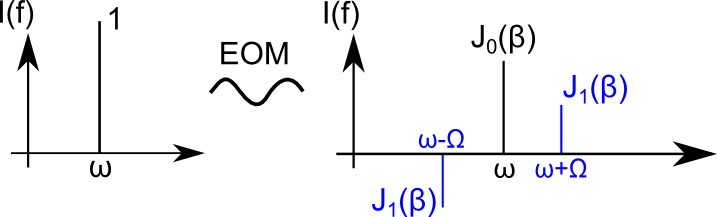
\includegraphics[scale=1.2]{spectrum.pdf}
  \caption{Expected spectrum of beam after phase modulation, to the first
  sidebands. While possibly present and significant, further sidebands can
  be ignored as they will be filtered during mixing.}
  \label{fig:eom_spectrum}
\end{figure}

\subsection{Error Signal Generation}

Obtaining an accurate value for the optimal error signal slope will be a central
development task, if it is not possible to obtain heuristically in
a way that is comfortable for the laboratory staff. Rigorous analysis will
involve some complex quantum mechanical models, but there are precedents for
reference \cite{maguire2006}. \\

The entire PDH error-signal generating setup is depicted in
\textbf{ Figure \ref{fig:setup}}.
The master laser enters at the left, and is immediately split by a
polarizing cube into two beams.  The lower "pump" beam (dashed line), unmodified,
reflects off of several mirrors, and is directed into a chamber full of
Rubidium gas. This beam serves to saturate the absorption ability of the gas,
which results in the a set of Doppler-cancelled features.
The most predominant of these features is used as a locking point. \\

The second "probe" beam is passed into an EOM.  This modulator is fed by a VCO,
running at frequency $\Omega$. As previously discussed, this creates the spectrum
shown in \textbf{Figure \ref{fig:eom_spectrum}}. After being passed through the
vapour cell, the amplitudes of the carrier and the sidebands are attenuated
according to the transmission profile of the saturated absorption feature,
of which a naive representation is shown in
\textbf{Figure \ref{fig:rb87d2abs}}. Let $\hat{F}$ be the operator that
describes the attentuation of the probe beam as it passes through the
vapour cell. Then, the resultant beam is, to the first sidebands:
\begin{gather}
  E_0 e^{i \omega t + \beta \sin \Omega t} \xrightarrow{\hat{F}}
    E_0e^{i \omega t }\left( J_0(\beta)\hat{F}(\omega) +
      J_1(\beta)\hat{F}(\omega + \Omega)e^{i\Omega t} +
        J_1(\beta)\hat{F}(\omega - \Omega)e^{-i\Omega t} \right)
\end{gather}

\begin{figure}
  \centering
  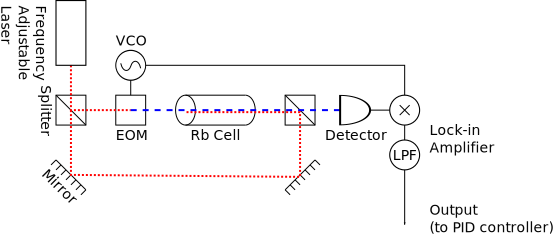
\includegraphics[scale=0.95]{setup.pdf}
  \caption{High level layout of the proposed PDH servo loop using a Rubidium
   vapour cell as the frequency selective element.}
    \label{fig:setup}
\end{figure}

This beam is then coupled into a high-speed fiber optic receiver, a
photosensor unit with bandwidth up to 12GHz. The current produced by the
biased sensor is proportional to the incident optical power. As
$P = |E|^2$, this creates a signal with some mixed frequency components. After
applying a low pass filter to this signal, with a pole at $\sim 1.5 \Omega$,
the following waveform is extracted:
\begin{gather}
  V_1(t) = A(\hat{F}, \omega, \Omega) E_0^2 +
    E_0^2 (J_0(\beta)J_1(\beta))
    (\hat{F}(\omega + \Omega) - \hat{F}(\omega - \Omega))cos(\Omega t)
\end{gather}

Where  $A(\hat{F}, \omega, \Omega)$ is some down-mixed DC term that is dependent
on carrier and side-band powers, as well as the frequency selective element
(it will be filtered out shortly). It is clear even at this stage, that being
able to isolate $(\hat{F}(\omega + \Omega) - \hat{F}(\omega - \Omega))$ will
provide some variable accuracy estimation of the \emph{derivative} of the
saturated absorption spectrum, and will provide a convenient null locking point
at any absorption peaks, which are located at important resonances. To extract
this value explicitly, $V_1$ is mixed with a phase delayed version of the
VCO signal, of frequency $\Omega$ and filtered to extract the DC error signal,
which is explicitly:
\begin{gather}\label{eq:err_sig}
  \epsilon = \alpha E_0^2 (J_0(\beta)J_1(\beta))
    (\hat{F}(\omega + \Omega) - \hat{F}(\omega - \Omega))\cos\phi
\end{gather}
where $\alpha$ is some attentuation factor, dependent on electrical components,
and $\phi$ is the phase delay between the oscillator signal being mixed
and the oscillator signal driving the EOM (same source, one passes through
extra cabling and other components such as buffers, etc). It is clear that
care must be taken to select an appropriate $\phi$ so as to generate a
clear, useable error signal. $\epsilon$ is then fed back into the
laser controller and used to sweep $\omega$ as necessary.
An example error signal, using the naive Rb87 D2 profile in
\textbf{Figure \ref{fig:rb87d2abs}} and generated with different phase modulation
frequencies to show the change in slope about the lock point is shown in
\textbf{Figure \ref{fig:err_gen}\subref*{fig:error_far}}, with an explicit
change in the slope made clear in
\textbf{Figure  \ref{fig:err_gen}\subref*{fig:error_close}}. It is clear from
this analysis that, for this particular absorption profile,
there exists some $\Omega$ between 100kHz and 10MHz that produces
the maximum error signal slope. Maximizing the slope is important as it provides
the smallest drift in frequency for a given change in signal voltage, which
allows any locking system to lock closer to the resonance, given a particular
voltage resolution. If the absorption spectrum for the Rb87 D2 transition has
similar feature size, then it is clear that the existing AOM solution is,
at best, suboptimal.

\begin{figure}
  \begin{tabularx}{\linewidth}{c}
    \subfloat[View far from the null lock point, showing the entire
    feature and generated error signals.]
    {
      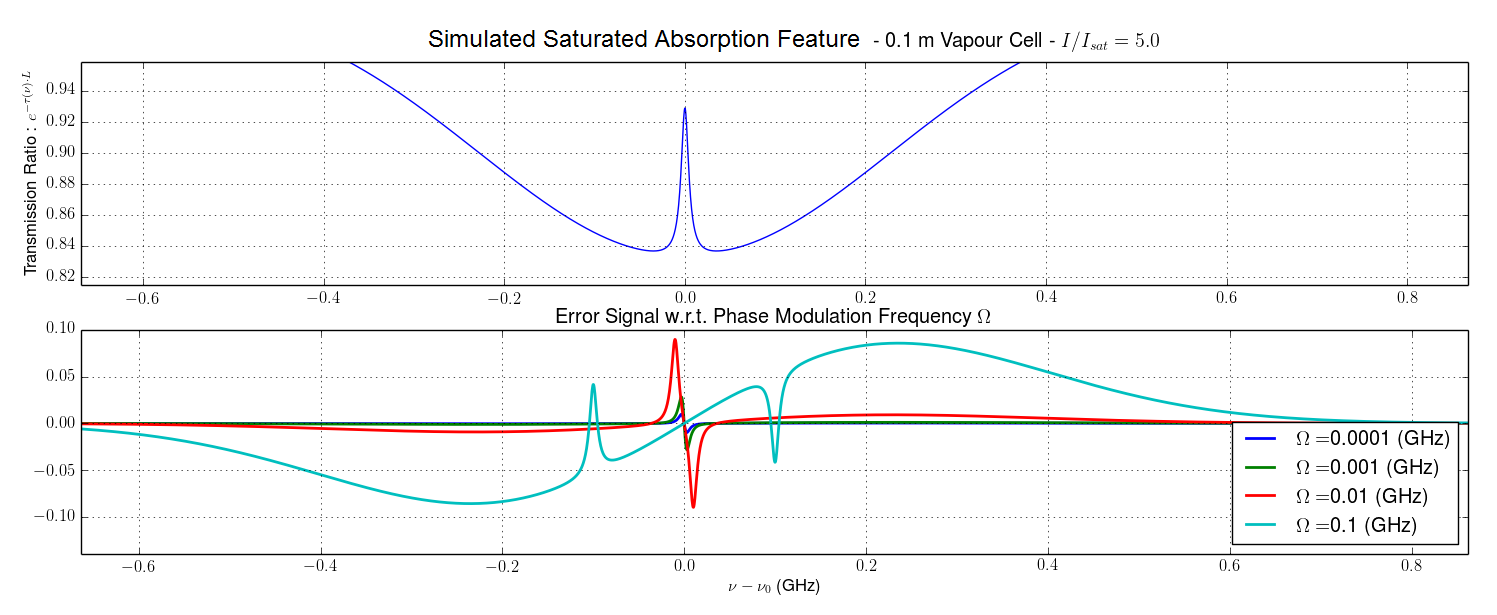
\includegraphics[height=0.5\linewidth, width=\linewidth]
        {rb_D2_error_faraway.png}
      \label{fig:error_far}
    } \\
    \subfloat[View close to the  null lock point, showing the change in
    slope about it as $\Omega$ is varied.]
    {
      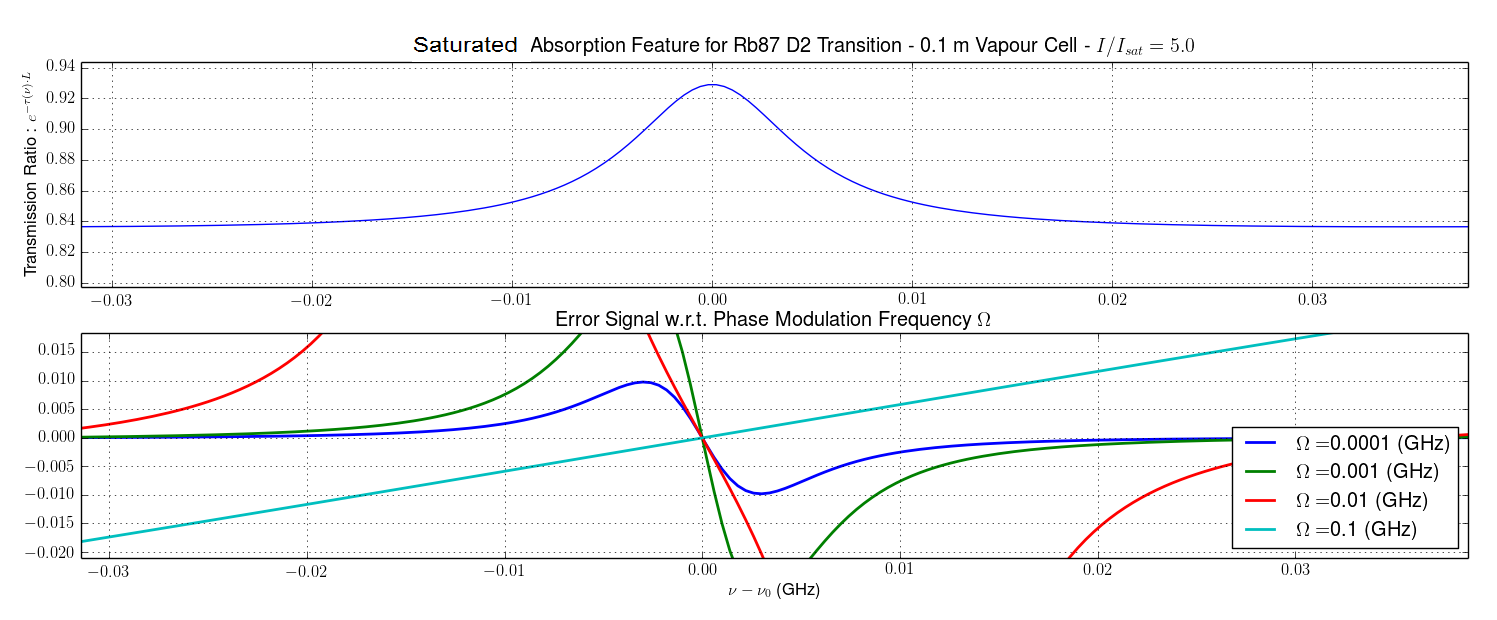
\includegraphics[height=0.5\linewidth, width=\linewidth]
        {rb_D2_error_closer.png}
      \label{fig:error_close}
    }
  \end{tabularx}
  \caption{Generation of an error signal with varying modulation frequencies
    / sideband separation $\Omega$, using (\ref{eq:err_sig}), for a
    saturated absorption feature generated with (\ref{eq:corr_opt_depth}).
    It is clear,
    especially in \protect\subref{fig:error_close}, that there is some
    optimal value for $\Omega$ that creates the largest slope about the
    null lock point. This value will be highly dependent on the size
    of locking features in the saturated absorption spectrum. }
  \label{fig:err_gen}
\end{figure}


%%%%%%%%%%%%%%%% IMPLEMENTATION

\newpage
\section{Implementation}

Mention how we modified the EOM driver to run off of the same lab power supply to eliminate unwanted coupling. \\

EOM driver onboard phase shift is bad, (see figure) only allowing for shifts between $\lambda \in [0.23, 0.41]$. However, for reasons unknown, this onboard system simulatneously introduced some low-frequency noise which propagated through to the error signal. The frequency was left at 19.8 MHz with no onboard phase delay as it produced the strongest and cleanest error signal. Phase delay was instead accomplished using variable length 50$\Omega$ BNC cables, with a 1.5m cable producing the strongest signal. \\

\begin{figure}
  \begin{tabular}{cc}
    \includegraphics[width=0.47\textwidth]{figures/{eom_driver_onboard_1}.jpg} &
    \includegraphics[width=0.47\textwidth]{figures/{eom_driver_onboard_2}.jpg} \\
  \end{tabular}
  \caption{Measuring the maximum phase shift of the EOM driver reference output. Depending on the impedance characteristics of the load, either or both waveforms would change in amplitude and spectral quality.}
\end{figure}

Using the fitted MHz/s parameters, we can see that for $^{87}$Rb and $^{85}$Rb, the ramping was done at approximately $115 \pm 4 Mhz/s$ and $140 \pm 3 Mhz/s$, respectively.

Originally tried beam sizes from that paper, but introducing 3:1 telescopes on either side of the cell drastically improved SNR.

\subsection{Overview}

\subsection{Laser Slave Seeding}

The laser setup begins with the master laser, a rubidium laser [details?].  This laser feeds its light into a ``slave'' laser, which stimulates emission at the same frequency by the second laser.

That slave then feeds into *another* slave, which we have direct access to.  Particularly, there are a series of mirrors which direct the light from the second slave into the third slave.  Setting up this slave requires a particular algorithm (must be done at the beginning of each day):

 1. Lock the master laser and first slave.  This is somewhat involved, but beyond the scope of this document.
 2. Set the current on this slave to a low value, typically 32.0mA is used.
 3. Place a power meter at the output of this slave laser.
 4. Adjust the two mirrors feeding master light into the slave, until the power output from the slave laser is maximised.
 5. Unlock the master laser.  Set it to sweep frequency across a wide enough range that the Rb85 and Rb87 absorbtion features [which ones, specifically?] are visible on the master's diagnostic scope.
 6. Make sure that light from the slave laser is fed back to the diagnostic table (via fibre coupling).  Check with the power meter that >50\% of the slave light is entering the fibre (there are many reasons why the light might not make it this far.
 7. Set the current into the slave to a high value (110.0mA), and gradually decrease it.  Observe that there is a "stable" frequency window in which the slave can operate, and that adjusting the current moves this window.  Reduce the current of the slave until the feature of interest is in the centre of the stability window.  The window should be wide enough to contain both the Rb85 and Rb87 transitions.
 8. The laser can now be used for experiments.

\subsection{Laser sweeping}

The master laser is nominally operated in a "locked-frequency" mode.  There is a "lock-box" which provides this function, and an AOM-based locking system.  This provides a fast (current-based) and slow (piezo-based) feedback response to the laser's frequency.

However, if we disable the feedback, we can operate the lockbox in a "frequency sweeping" mode, in which no locking is performed.  The lock box does not touch the current, but it slowly moves the piezo element in a triangular wave.  This directly affects the frequency output of the master laser, giving us a frequency sweep which is very slow compared to the locking system, but fast enough to give a continuous view of how the system responds in frequency.

Particularly, by using this triangular wave as the trigger on an oscilloscope, we get a continuously-updating view of the frequency response of our system.  Frequency appears on the x-axis, and the quantity of interest appears on the y-axis.  For example, by sending this beam through a Rb gas cell, and placing a detector on the far side, we get a plot of the absorbtion spectrum of rubidium against frequency.

If we plot the DC value of our system on the y-axis, then we observe the strength of the feedback signal as a function of frequency.

\subsection{Alignment}

In short, lots!  Each beam has four degrees of freedom.  Thus aligning the beams (in two axes) in two locations is sufficient to have the beams perfectly aligned.  This is required for both fibre couplers and cavities.

Fibre couplers:

 1. Use the "spaghetti laser" to create a narrow beam coming out of the fibre.  This will be used to determine the alignment of the coupler.
 2. Place a transparent IR card near the fibre coupler such that you can see both the spaghetti laser beam, and the slave laser beam.
 3. Adjust the last mirror before the coupler until these two beams line up precisely.
 4. Place the transparent IR card past the last mirror [TODO(jeff) figure].
 5. Adjust the fibre coupler until the two beams line up.
 6. Remove the spaghetti laser and IR card.  Attach the power meter to the fibre coupler.  You should see some power.
 7. Adjust the same four degrees of freedom on the mirror and coupler, maximising the power entering the fibre coupler.  These should be small adjustments.

Talk about cavities or is this too much?
 
\subsection{Pump/Probe, Saturated Absorption}

- We feed the an EOM-modulated beam into the sample from the right to left.  A beam passes through the gas from left to right, and the signal is "written" across the beams selectively when the laser is near the transition frequnecy.

\subsection{EOM + Crystal Driver + Power Supply}

An EOM crystal driver (used for the PHYS 408 labs) was provided.  This generates a ~20MHz signal, and is tuned to drive the high capacitance of the EOM crystal at a high voltage.

This board came with an AC-DC wall wart.  However, supply noise proved to be a problem, so a custom power supply was developed for this board.  The power supply takes filtered DC lab power, and linearly downregulates to the needed input power [TODO elaborate]

\subsection{Cavity EOM measurement}

- A confocal cavity was used to measure the effect the EOM has on the beam, to ensure that sidebands are in fact being created.  The cavity resonates more highly with laser light that fits in an integer number of wavelengths within the cavity.  Having a photodiode on the end allows us to measure the amplitude of that resonance.  The backside of the cavity can be moved by adjusting the voltage applied to a piezo system.  By feeding a triangular wave in (from a function generator), we can observe the (rough) frequency spectrum of the beam.

[confocal cavity]

This allows us to measure that the EOM driver is, in fact functioning.  However, the frequency resolution of this instrument is about 10MHz [include math!] at best.  This means that our 20MHz features are only *barely* resolvable.

\subsection{Heated Rb Cell}

For the tests that including temperature control, a heating element was used.  This consists of a thermistor (to measure temperature) and several heating pads, attached to a DC power supply.

During these tests, the current output was manually controlled, until the thermistor's reading had been stable for several minutes.  Then the power was switched off, and the measurements recorded.

\subsection{Saturated Abosorbtion Measurement}

Since the frequency was sweeping during our main tests, we incorporated a low-frequency detector to give us an indication of how our rubidium cell was responding to the input beam, possible with saturated absorbtion.  This proved to be very useful.

We later replaced the low-frequency thorlabs detector with an in-house detector (the "fat" detector), which performed better, and works well both at DC and RF.  We isolated the two signals before later processing.

\subsection{Error signal (20Mhz) Detection}

TODO

- Originally using ROSA.  Later replaced by "fat" detector, which provides stronger signal at both DC and 20MHz.

NOTE: Doesn't belong here, but the ROSA detector includes some 10kHz sidebands on the error signal, which contribute significantly (only a few dB below carrier) to the output.  Need to talk about these.  Origin unknown, possibly IM3 (nonlinearities) in detector.  Present *before* amplification, and not in the "fat" detector signal, so unique to ROSA.  Also only exist when beam+EOM are on.

\subsection{Signal Conditioning Case}

A custom case was designed and constructed for the custom electronics in the project.  It contains a central power distributor, which downregulates ±15V DC lab power to ±5V DC power taken by the amplifiers.

\subsection{Preamplification}

The 20MHz signal created at the detector is first filtered.  This cuts out the DC component, which is used to measure the saturated absorbtion, and high frequency components, which are additional unwanted artefacts.  It leaves just a 20MHz signal.  We pass that signal through two minicircuits [partno] amplifiers, which increase the power level of the signal enough to make it usable.

\subsection{Demodulation (lock-in)}

The preamplified signal is passed into a frequency mixer.  That signal is mixed with the 20MHz local oscillator (the EOM driver).  The mixed signal is then filtered at 10MHz.  This eliminates high frequency components, and isolates a DC signal which tells us how far away from the set-point we are.  The selection of frequency is important at this stage.  The higher a frequency we chose, the faster our system can respond to changes in the laser, however, the higher the frequency, the more noise is present in the output.  We chose 10MHz, which is as fast as possible.  Reducing this cutoff would reduce the output noise further.

\subsection{Laser Diode Feedback (not implemented)}

In order for the system to actually be used, the feedback loop would need to be closed.  That is, the demodulated error signal would need to be fed back into a laser diode controller, which would use the signal to adjust the frequency of the laser itself.  A suitable solution available in the lab was the Vescent D2-105 laser controller, which includes fast (current) and slow (piezo) control, and a built in PI²D controller.  This was not implemented, as the sponsor indicated that they would prefer a deeper investigation of possible tactics to improve the error signal, over closing the loop and providing a functional (but sub-optimal) solution.






%%%%%%%%%%%%%%%% IMPLEMENTATION

\newpage
\section{Validation}

\subsection{Data Analysis}

Peak finding error in establishing MHz/s scales for all plots. Mention that temperature data got pretty useless pretty fast.

Technique for finding slope about lock points. Don't need pictures, just mention it.

Peak Drift thing


%%%%%%%%%%%%%%%% DELIVERABLES

\newpage
\section{Deliverables}

%%%%%%%%%%%%%%%% RECOMMENDATIONS

\newpage

\section{Recommendations}

\subsection{Improved Phase Adjustment}

Our current understanding of modulation transfer spectroscopy indicates that the position of the zero crossing is independant of the phase adjustment.  However, the amplitude of the signal is not.  This parameter is fairly easy to optimize, but the current phase adjustment scheme does not work very well.  Implementing an improved phase adjustment which allows a full 180° would make this optimization much easier to do.

\subsection{EOM driving frequencies}

The features in the Rb85 transitions are roughly 30MHz apart.  With a 20MHz EOM driver signal, we notice that the fringes of two strong signals overlap, crossing zero at a crossover.  If a 30MHz EOM driver were used instead, these two signals might constructively amplify, creating a very clean error signal.

An alternative approach uses the Rb87 features, which are generally more separated from one another.  Since our oscillator was fixed in frequency, we didn't get to experiment with the effect of the driving frequency on the quality of the error signal.

\subsection{Laser Power}

The best quality measurement we made was using 100\% of our laser's power.  Thus, it is possible that by increasing the power even further, an even-better signal-to-noise ratio could be achieved.

\subsection{Improved pre-amplifiers}

Near the end of the project, we decided that reducing noise was our priority.  The first and foremost concern is the noise from the amplifiers themselves.  The amplifiers we used, the ZFL-1000+, also exists in a low noise variant, the ZFL-1000LN+.  This amplifier has nearly identical properties, but the noise figure is lower, 3dB instead of 6dB \footnote{Noise figure is the amount that the SNR is increased by the amplifier.  That is, if we have a -20dBm carrier, with -30dBm of noise, and we feed it into a +20dB amplifier with +6dB noise figure, we get out a signal with 0dBm carrier, and -14dBm of noise.  So our SNR goes from 10dB to 4dB.}

Additionally, the amplifiers we're using do not have the specifications we desire.  They are the most appropriate from the supplier we used (minicircuits), but they're still far over-specified.  These amplifiers are designed to work up to 1000MHz, whereas we only need operation up to 20MHz.  We also require only a very narrow bandwidth near 20MHz.  There are likely amplifiers better suited to this purpose.  If not, then one could probably be made which meets these specifications, and ideally, has very good performance.  See, for example TI's guide to RF op amp circuits\cite{ti_amps}.

\subsection{Additional Low-Pass Filtering}

A spectral analysis of our noise indicates that the energy distribution is flat in frequency, white noise, up to our low-pass cutoff frequency (10MHz).  A crude, but likely effective way to remove noise would be to bring in a lower low-pass filter, which would have the effect of "averaging" the error signal in time, reducing the amount of white noise, at the cost of response time.


\subsubsection{Close the Loop}

In order for the system to actually be used, the feedback loop would need to be closed.  That is, the demodulated error signal would need to be fed back into a laser diode controller, which would use the signal to adjust the frequency of the laser itself.  A suitable solution available in the lab was the Vescent D2-105 laser controller, which includes fast (current) and slow (piezo) control, and a built in PI²D controller.  This was not implemented, as the sponsor indicated that they would prefer a deeper investigation of possible tactics to improve the error signal, versus closing the loop and providing a functional (but sub-optimal) solution.





%%%%%%%%%%%%%%%% CONCLUSION

\newpage
\section{Conclusion}

The UBC Quantum Degenerate Gases Laboratory is currently using an acousto-optic modulator-based system to lock a diode laser to a specific frequency.  This system is frequency limited, and is incapable of providing the narrow linewidths that they require for their experiments. \\

\section*{Acknowledgements}
\addcontentsline{toc}{section}{Acknowledgements}

This project was aided immensely by the research staff in the UBC Quantum Degenerate Gases laboratory led by Dr. Kirk Madison. Dr. Madison provided direct guidence on theoretical matters and contributed significant physical resources. Gene Polovy and Will Gunton of the Madison Group were extremely helpful with the physical setup, and with locating equipment. Janelle van Dongen provided significant assistance with the laser control instrumentation and data acquisition. Further thanks goes to Dr. David Jones, Dr. Jim Booth, Mariusz Semczuk, Koko Yu, Kahan Dare and Kais Jooya for their suggestions and guidance.

%%%%%%%%%%%%%%%% APPENDICES

\newpage
\section*{Appendix}
\addcontentsline{toc}{section}{Appendix}
\renewcommand{\thesubsection}{\Alph{subsection}}

\subsection{$^{85}$Rb Error Signals - Variable Power}
%
%   0.5mW Probe
%
\begin{figure}[H]
  \begin{tabular}{cc}
    \includegraphics[width=0.47\textwidth]{figures/{85_0.5mW_1.0mW}.png} &
    \includegraphics[width=0.47\textwidth]{figures/{85_0.5mW_2.0mW}.png} \\
    (a) Probe:Pump 0.5:1.0 (mW) & (b) Probe:Pump 0.5:2.0 (mW) \\[6pt]
    \includegraphics[width=0.47\textwidth]{figures/{85_0.5mW_4.0mW}.png} &
    \includegraphics[width=0.47\textwidth]{figures/{85_0.5mW_10.5mW}.png} \\
    (c) Probe:Pump 0.5:4.0 (mW) & (d) Probe:Pump 0.5:10.5 (mW) \\[6pt]
  \end{tabular}
  \caption{Modulation transfer spectroscopy error signals near the $^{85}$Rb $\left|F=3\right\rangle$ with 0.5 mW probe power and variable pump power. Effective 1/e beam waists inside the cell are approximately 4.0 mm for both beams.}
\end{figure}
\newpage
%
%   1.0mW Probe
%
\begin{figure}[H]
  \begin{tabular}{cc}
    \includegraphics[width=0.47\textwidth]{figures/{85_1.0mW_1.0mW}.png} &
    \includegraphics[width=0.47\textwidth]{figures/{85_1.0mW_2.0mW}.png} \\
    (a) Probe:Pump 1.0:1.0 (mW) & (b) Probe:Pump 1.0:2.0 (mW) \\[6pt]
    \includegraphics[width=0.47\textwidth]{figures/{85_1.0mW_4.0mW}.png} &
    \includegraphics[width=0.47\textwidth]{figures/{85_1.0mW_10.1mW}.png} \\
    (c) Probe:Pump 1.0:4.0 (mW) & (d) Probe:Pump 1.0:10.1 (mW) \\[6pt]
  \end{tabular}
  \caption{Modulation transfer spectroscopy error signals near the $^{85}$Rb $\left|F=3\right\rangle$ transitions with 1.0 mW probe power and variable pump power. Effective 1/e beam waists inside the cell are approximately 4.0 mm for both beams.}
\end{figure}
\newpage
%
%   2.0mW Probe
%
\begin{figure}[H]
  \begin{tabular}{cc}
    \includegraphics[width=0.47\textwidth]{figures/{85_2.0mW_1.0mW}.png} &
    \includegraphics[width=0.47\textwidth]{figures/{85_2.0mW_2.0mW}.png} \\
    (a) Probe:Pump 2.0:1.0 (mW) & (b) Probe:Pump 2.0:2.0 (mW) \\[6pt]
    \includegraphics[width=0.47\textwidth]{figures/{85_2.0mW_4.0mW}.png} &
    \includegraphics[width=0.47\textwidth]{figures/{85_2.0mW_9.3mW}.png} \\
    (c) Probe:Pump 2.0:4.0 (mW) & (d) Probe:Pump 2.0:9.3 (mW) \\[6pt]
  \end{tabular}
  \caption{Modulation transfer spectroscopy error signals near the $^{85}$Rb $\left|F=3\right\rangle$ transitions with 2.0 mW probe power and variable pump power. Effective 1/e beam waists inside the cell are approximately 4.0 mm for both beams.}
\end{figure}
\newpage
%
%   4.0mW Probe
%
\begin{figure}[H]
  \begin{tabular}{cc}
    \includegraphics[width=0.47\textwidth]{figures/{85_4.0mW_1.0mW}.png} &
    \includegraphics[width=0.47\textwidth]{figures/{85_4.0mW_2.0mW}.png} \\
    (a) Probe:Pump 4.0:1.0 (mW) & (b) Probe:Pump 4.0:2.0 (mW) \\[6pt]
    \includegraphics[width=0.47\textwidth]{figures/{85_4.0mW_4.0mW}.png} &
    \includegraphics[width=0.47\textwidth]{figures/{85_4.0mW_7.7mW}.png} \\
    (c) Probe:Pump 4.0:4.0 (mW) & (d) Probe:Pump 4.0:7.7 (mW) \\[6pt]
  \end{tabular}
  \caption{Modulation transfer spectroscopy error signals near the $^{85}$Rb $\left|F=3\right\rangle$ transitions with 4.0 mW probe power and variable pump power. Effective 1/e beam waists inside the cell are approximately 4.0 mm for both beams.}
\end{figure}
\newpage
%
%   6.0mW Probe
%
\begin{figure}[H]
  \begin{tabular}{cc}
    \includegraphics[width=0.47\textwidth]{figures/{85_6.0mW_1.0mW}.png} &
    \includegraphics[width=0.47\textwidth]{figures/{85_6.0mW_2.0mW}.png} \\
    (a) Probe:Pump 6.0:1.0 (mW) & (b) Probe:Pump 6.0:2.0 (mW) \\[6pt]
    \includegraphics[width=0.47\textwidth]{figures/{85_6.0mW_4.0mW}.png} &
    \includegraphics[width=0.47\textwidth]{figures/{85_6.0mW_6.0mW}.png} \\
    (c) Probe:Pump 6.0:4.0 (mW) & (d) Probe:Pump 6.0:6.0 (mW) \\[6pt]
  \end{tabular}
  \caption{Modulation transfer spectroscopy error signals near the $^{85}$Rb $\left|F=3\right\rangle$ transitions with 6.0 mW probe power and variable pump power. Effective 1/e beam waists inside the cell are approxximately 4.0 mm for both beams.}
\end{figure}
\newpage

\subsection{$^{85}$Rb Error Signals - Variable Temperature}
\begin{figure}[H]
  \begin{tabular}{cc}
    \includegraphics[width=0.47\textwidth]{figures/{85_40C}.png} &
    \includegraphics[width=0.47\textwidth]{figures/{85_60C}.png} \\
    (a) 40$^{\circ}$ C & (b) 60$^{\circ}$ C  \\[6pt]
    \includegraphics[width=0.47\textwidth]{figures/{85_80C}.png} &
    \includegraphics[width=0.47\textwidth]{figures/{85_102C}.png} \\
    (c) 80$^{\circ}$ C  & (d) 102$^{\circ}$ C  \\[6pt]
  \end{tabular}
  \caption{Modulation transfer spectroscopy error near the $^{87}$Rb $\left|F=2\right\rangle$ transitions with varying temperature. Pump and probe beam power were both held at a constant 4.0 mW. Effective 1/e beam waists inside the cell are approximately 4.0 mm for both beams. Past 60$^{\circ}$, the spectrum rapidly beacame unusable due to pressure broadening.}
\end{figure}
\newpage

\subsection{$^{87}$Rb Error Signals - Variable Power}
%
%   0.5mW Probe
%
\begin{figure}[H]
  \begin{tabular}{cc}
    \includegraphics[width=0.47\textwidth]{figures/{87_0.5mW_1.0mW}.png} &
    \includegraphics[width=0.47\textwidth]{figures/{87_0.5mW_2.0mW}.png} \\
    (a) Probe:Pump 0.5:1.0 (mW) & (b) Probe:Pump 0.5:2.0 (mW) \\[6pt]
    \includegraphics[width=0.47\textwidth]{figures/{87_0.5mW_4.0mW}.png} &
    \includegraphics[width=0.47\textwidth]{figures/{87_0.5mW_10.4mW}.png} \\
    (c) Probe:Pump 0.5:4.0 (mW) & (d) Probe:Pump 0.5:10.4 (mW) \\[6pt]
  \end{tabular}
  \caption{Modulation transfer spectroscopy error signals near the $^{87}$Rb $\left|F=2\right\rangle$ with 0.5 mW probe power and variable pump power. Effective 1/e beam waists inside the cell are approximately 4.0 mm for both beams.}
\end{figure}
\newpage
%
%   1.0mW Probe
%
\begin{figure}[H]
  \begin{tabular}{cc}
    \includegraphics[width=0.47\textwidth]{figures/{87_1.0mW_1.0mW}.png} &
    \includegraphics[width=0.47\textwidth]{figures/{87_1.0mW_2.0mW}.png} \\
    (a) Probe:Pump 1.0:1.0 (mW) & (b) Probe:Pump 1.0:2.0 (mW) \\[6pt]
    \includegraphics[width=0.47\textwidth]{figures/{87_1.0mW_4.0mW}.png} &
    \includegraphics[width=0.47\textwidth]{figures/{87_1.0mW_9.9mW}.png} \\
    (c) Probe:Pump 1.0:4.0 (mW) & (d) Probe:Pump 1.0:9.9 (mW) \\[6pt]
  \end{tabular}
  \caption{Modulation transfer spectroscopy error signals near the $^{87}$Rb $\left|F=2\right\rangle$ transitions with 1.0 mW probe power and variable pump power. Effective 1/e beam waists inside the cell are approximately 4.0 mm for both beams.}
\end{figure}
\newpage
%
%   2.0mW Probe
%
\begin{figure}[H]
  \begin{tabular}{cc}
    \includegraphics[width=0.47\textwidth]{figures/{87_2.0mW_1.0mW}.png} &
    \includegraphics[width=0.47\textwidth]{figures/{87_2.0mW_2.0mW}.png} \\
    (a) Probe:Pump 2.0:1.0 (mW) & (b) Probe:Pump 2.0:2.0 (mW) \\[6pt]
    \includegraphics[width=0.47\textwidth]{figures/{87_2.0mW_4.0mW}.png} &
    \includegraphics[width=0.47\textwidth]{figures/{87_2.0mW_9.3mW}.png} \\
    (c) Probe:Pump 2.0:4.0 (mW) & (d) Probe:Pump 2.0:9.3 (mW) \\[6pt]
  \end{tabular}
  \caption{Modulation transfer spectroscopy error signals near the $^{87}$Rb $\left|F=2\right\rangle$ transitions with 2.0 mW probe power and variable pump power. Effective 1/e beam waists inside the cell are approximately 4.0 mm for both beams.}
\end{figure}
\newpage
%
%   4.0mW Probe
%
\begin{figure}[H]
  \begin{tabular}{cc}
    \includegraphics[width=0.47\textwidth]{figures/{87_4.0mW_1.0mW}.png} &
    \includegraphics[width=0.47\textwidth]{figures/{87_4.0mW_2.0mW}.png} \\
    (a) Probe:Pump 4.0:1.0 (mW) & (b) Probe:Pump 4.0:2.0 (mW) \\[6pt]
    \includegraphics[width=0.47\textwidth]{figures/{87_4.0mW_4.0mW}.png} &
    \includegraphics[width=0.47\textwidth]{figures/{87_4.0mW_7.6mW}.png} \\
    (c) Probe:Pump 4.0:4.0 (mW) & (d) Probe:Pump 4.0:7.6 (mW) \\[6pt]
  \end{tabular}
  \caption{Modulation transfer spectroscopy error signals near the $^{87}$Rb $\left|F=2\right\rangle$ transitions with 4.0 mW probe power and variable pump power. Effective 1/e beam waists inside the cell are approximately 4.0 mm for both beams.}
\end{figure}
\newpage
%
%   6.0mW Probe
%
\begin{figure}[H]
  \begin{tabular}{cc}
    \includegraphics[width=0.47\textwidth]{figures/{87_6.0mW_1.0mW}.png} &
    \includegraphics[width=0.47\textwidth]{figures/{87_6.0mW_2.0mW}.png} \\
    (a) Probe:Pump 6.0:1.0 (mW) & (b) Probe:Pump 6.0:2.0 (mW) \\[6pt]
    \includegraphics[width=0.47\textwidth]{figures/{87_6.0mW_4.0mW}.png} &
    \includegraphics[width=0.47\textwidth]{figures/{87_6.0mW_5.8mW}.png} \\
    (c) Probe:Pump 6.0:4.0 (mW) & (d) Probe:Pump 6.0:5.8 (mW) \\[6pt]
  \end{tabular}
  \caption{Modulation transfer spectroscopy error signals near the $^{87}$Rb $\left|F=2\right\rangle$ transitions with 6.0 mW probe power and variable pump power. Effective 1/e beam waists inside the cell are approxximately 4.0 mm for both beams.}
\end{figure}
\newpage

\subsection{$^{87}$Rb Error Signals - Variable Temperature}
\begin{figure}[H]
  \begin{tabular}{cc}
    \includegraphics[width=0.47\textwidth]{figures/{87_40C}.png} &
    \includegraphics[width=0.47\textwidth]{figures/{87_60C}.png} \\
    (a) 40$^{\circ}$ C & (b) 60$^{\circ}$ C  \\[6pt]
    \includegraphics[width=0.47\textwidth]{figures/{87_80C}.png} &
    \includegraphics[width=0.47\textwidth]{figures/{87_100C}.png} \\
    (c) 80$^{\circ}$ C  & (d) 100$^{\circ}$ C  \\[6pt]
  \end{tabular}
  \caption{Modulation transfer spectroscopy error near the $^{87}$Rb $\left|F=2\right\rangle$ transitions with varying temperature. Pump and probe beam power were both held at a constant 4.0 mW. Effective 1/e beam waists inside the cell are approximately 4.0 mm for both beams. As with the $^{85}$Rb data, the spectrum rapidly beacame unusable past 60$^{\circ}$C due to pressure broadening.}
\end{figure}
\newpage

\subsection{Probe Modulated Saturated Absorption Error Signal}

\subsection{Pump Modulated Modulation Transfer Error Signal}

\subsection{Phase Response Measurements in Rubidium}

%%%%%%%%%%%%%%%% REFERENCES

\newpage
\printbibliography

\end{document}



